\documentclass[a4paper,12pt]{extarticle}
\usepackage[margin=1.5cm]{geometry}
\usepackage{amsmath, amssymb}
\usepackage{array}
\usepackage{multicol}
\usepackage{helvet}
\usepackage{multirow}
\usepackage{graphicx}
\renewcommand{\baselinestretch}{2}
\renewcommand{\familydefault}{\sfdefault}

\begin{document}

    \begin{tabular}{| c | c | c | c |}
        \hline
        & MATEMÁTICAS & 18/03/2026 & calificación \\
        \hline 

        \multirow{2}{*}{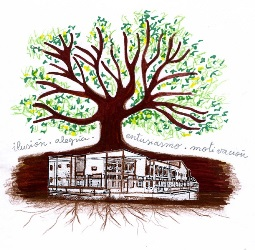
\includegraphics{../../img-Logos/iesoGalileo.jpg}} & Nombre y apellidos \hspace{120pt} & Ex. 3º ESO UD5:  & \\ 
        &&Sistemas de Ecuaciones& \\ 
        \hline
    \end{tabular}
    
    \begin{tabular}{| l | }
        \hline
        NOTAS: \\ 
            1. El examen tiene que ser limpio, ordenado y sin faltas de ortografía. \\
            
            2. El examen ha de realizarse en bolígrafo negro o azul, evitando tachones en la medida \\
            de lo posible. \\ 
            
            3. Deben aparecer todas las operaciones NO vale con indicar solo el resultado.\\
            
            4. Los problemas deben contener: Datos, planteamiento y resolución, respondiendo a lo \\
            que se pregunte, NO vale con indicar un número como solución del problema.\\

            5. Persona que se vea copiando o hablando con un compañero tiene un cero en el examen\\
        \hline
    \end{tabular}

    \begin{enumerate}
        \item (0,5 puntos) Indica cuál de estas ecuaciones es lineal
            \begin{enumerate}
                \item $2x^3+y=5$
                \item $2xy-6=2$
                \item $2x+3y=x+y-6$
                \item $y^2-x=8$
            \end{enumerate}
        \item (0,5 puntos) Un Sistema es compatible indeterminado cuando tiene:
            \begin{enumerate}
                \item 0 soluciones
                \item 1 solución
                \item 2 soluciones
                \item Infinitas soluciones
            \end{enumerate}
    \newpage
        \item (0.5 puntos) Expresa mediante una ecuación con dos incógnitas la siguiente afirmación:
            \begin{enumerate}
                \item (0.25 puntos) La suma de dos números menos su diferencia es igual a 10. $\vspace{0.5cm}$ 
                \item (0.25 puntos) La mitad del producto de dos números es 120. $\vspace{0.5cm}$ 
            \end{enumerate}
        \item (0.5 puntos) Indica la solución al sistema: $\left \{\begin{array}{rr}
                    \dfrac{-x+y}{2}=4 \\
                    \dfrac{x}{4}+y=1+\dfrac{3y}{4}
                \end{array}\right .$

                \begin{enumerate}
                    \item (1,3)
                    \item (-2,6)
                    \item (1,9)
                \end{enumerate}
        \item (2 puntos) Resuelve el siguiente sistema
        
            $\left \{\begin{array}{rr}
                    x+3y=2 \\
                    -2x+3y=5
                \end{array}\right .$ $\vspace{5cm}$ 

                \newpage
        \item (2 puntos)Representa el siguiente sistema e indica cuál sería la solución.
        
        $\left \{\begin{array}{rr}
                -2x+y=1 \\
                x+2y=2
            \end{array}\right .$ 


        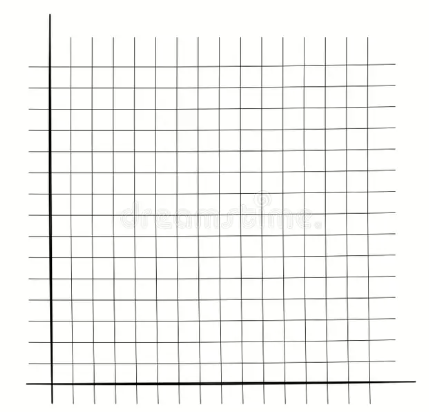
\includegraphics{img/cuadricula.png} 

        \item (2 puntos) En un patio de una escuela infantil hay triciclos y cochecitos. En total son 20 y todas las ruedas suman 67. ¿Cuántos triciclos y cuántos cochecitos hay en el patio?$\vspace{7cm}$ \newpage
        \item (2 puntos) Las edades de Esther y su padre suman 30 años. Dentro de 18 años, la edad de su padre será el soble que la de Esther ¿Cuántos años tiene cada uno? $\vspace{7cm}$ 
        \item EXTRA (1 punto) Halla el valor de $a$ y $b$ para que el par (3,-1) sea solución del sistema:
        
        $\left \{\begin{array}{rr}
                    ax+y=5 \\
                    -3x+by=-5
                \end{array}\right .$ 
    \end{enumerate}
\end{document}